
% This document is for the Group Meeting Agenda.  The Agenda should
% be distributed to each member (and other invitees) and to the TA
% prior to the meeting (hopefully the day before) so that each member
% will have adequate time to prepare for the meeting.  The best way
% to accomplish the distribution of the agenda is to email the LaTeX
% file to all members and TA.
%
%\documentstyle[fullpage]{article}
\documentclass[a4paper,12pt]{article}
\usepackage{fullpage}
\usepackage{cite}
\usepackage{url}
\usepackage{xcolor}
\usepackage{setspace}
\usepackage[version=4]{mhchem}
\usepackage{upgreek}
\usepackage[margin=0.75in]{geometry}
% For figure:
\usepackage{graphicx}
\usepackage{float}
% For table:
\usepackage{makecell}
\makeatletter
% we use \prefix@<level> only if it is defined
\renewcommand{\@seccntformat}[1]{%
  \ifcsname prefix@#1\endcsname
    \csname prefix@#1\endcsname
  \else
    \csname the#1\endcsname\quad
  \fi}
% define \prefix@section
\newcommand\prefix@section{}
\makeatother
\begin{document}

\title{Vertebrate Biodiversity
\author{"Reptiles"
\date{Fall 2020}
}}
\maketitle

%
% This section gives the general information about the meeting such
% as the title, who it was called by, when and where the meeting
% will take place, what type of meeting it is (planning, design,
% problem-solving, decision-making, etc.), and of course who is
% invited to attend.
%


\section{Amniota}
Egg equipped with amnion, chorion, and allantois membranes- adaptation for fully terrestrial living

\begin{figure}[H]
\centering
  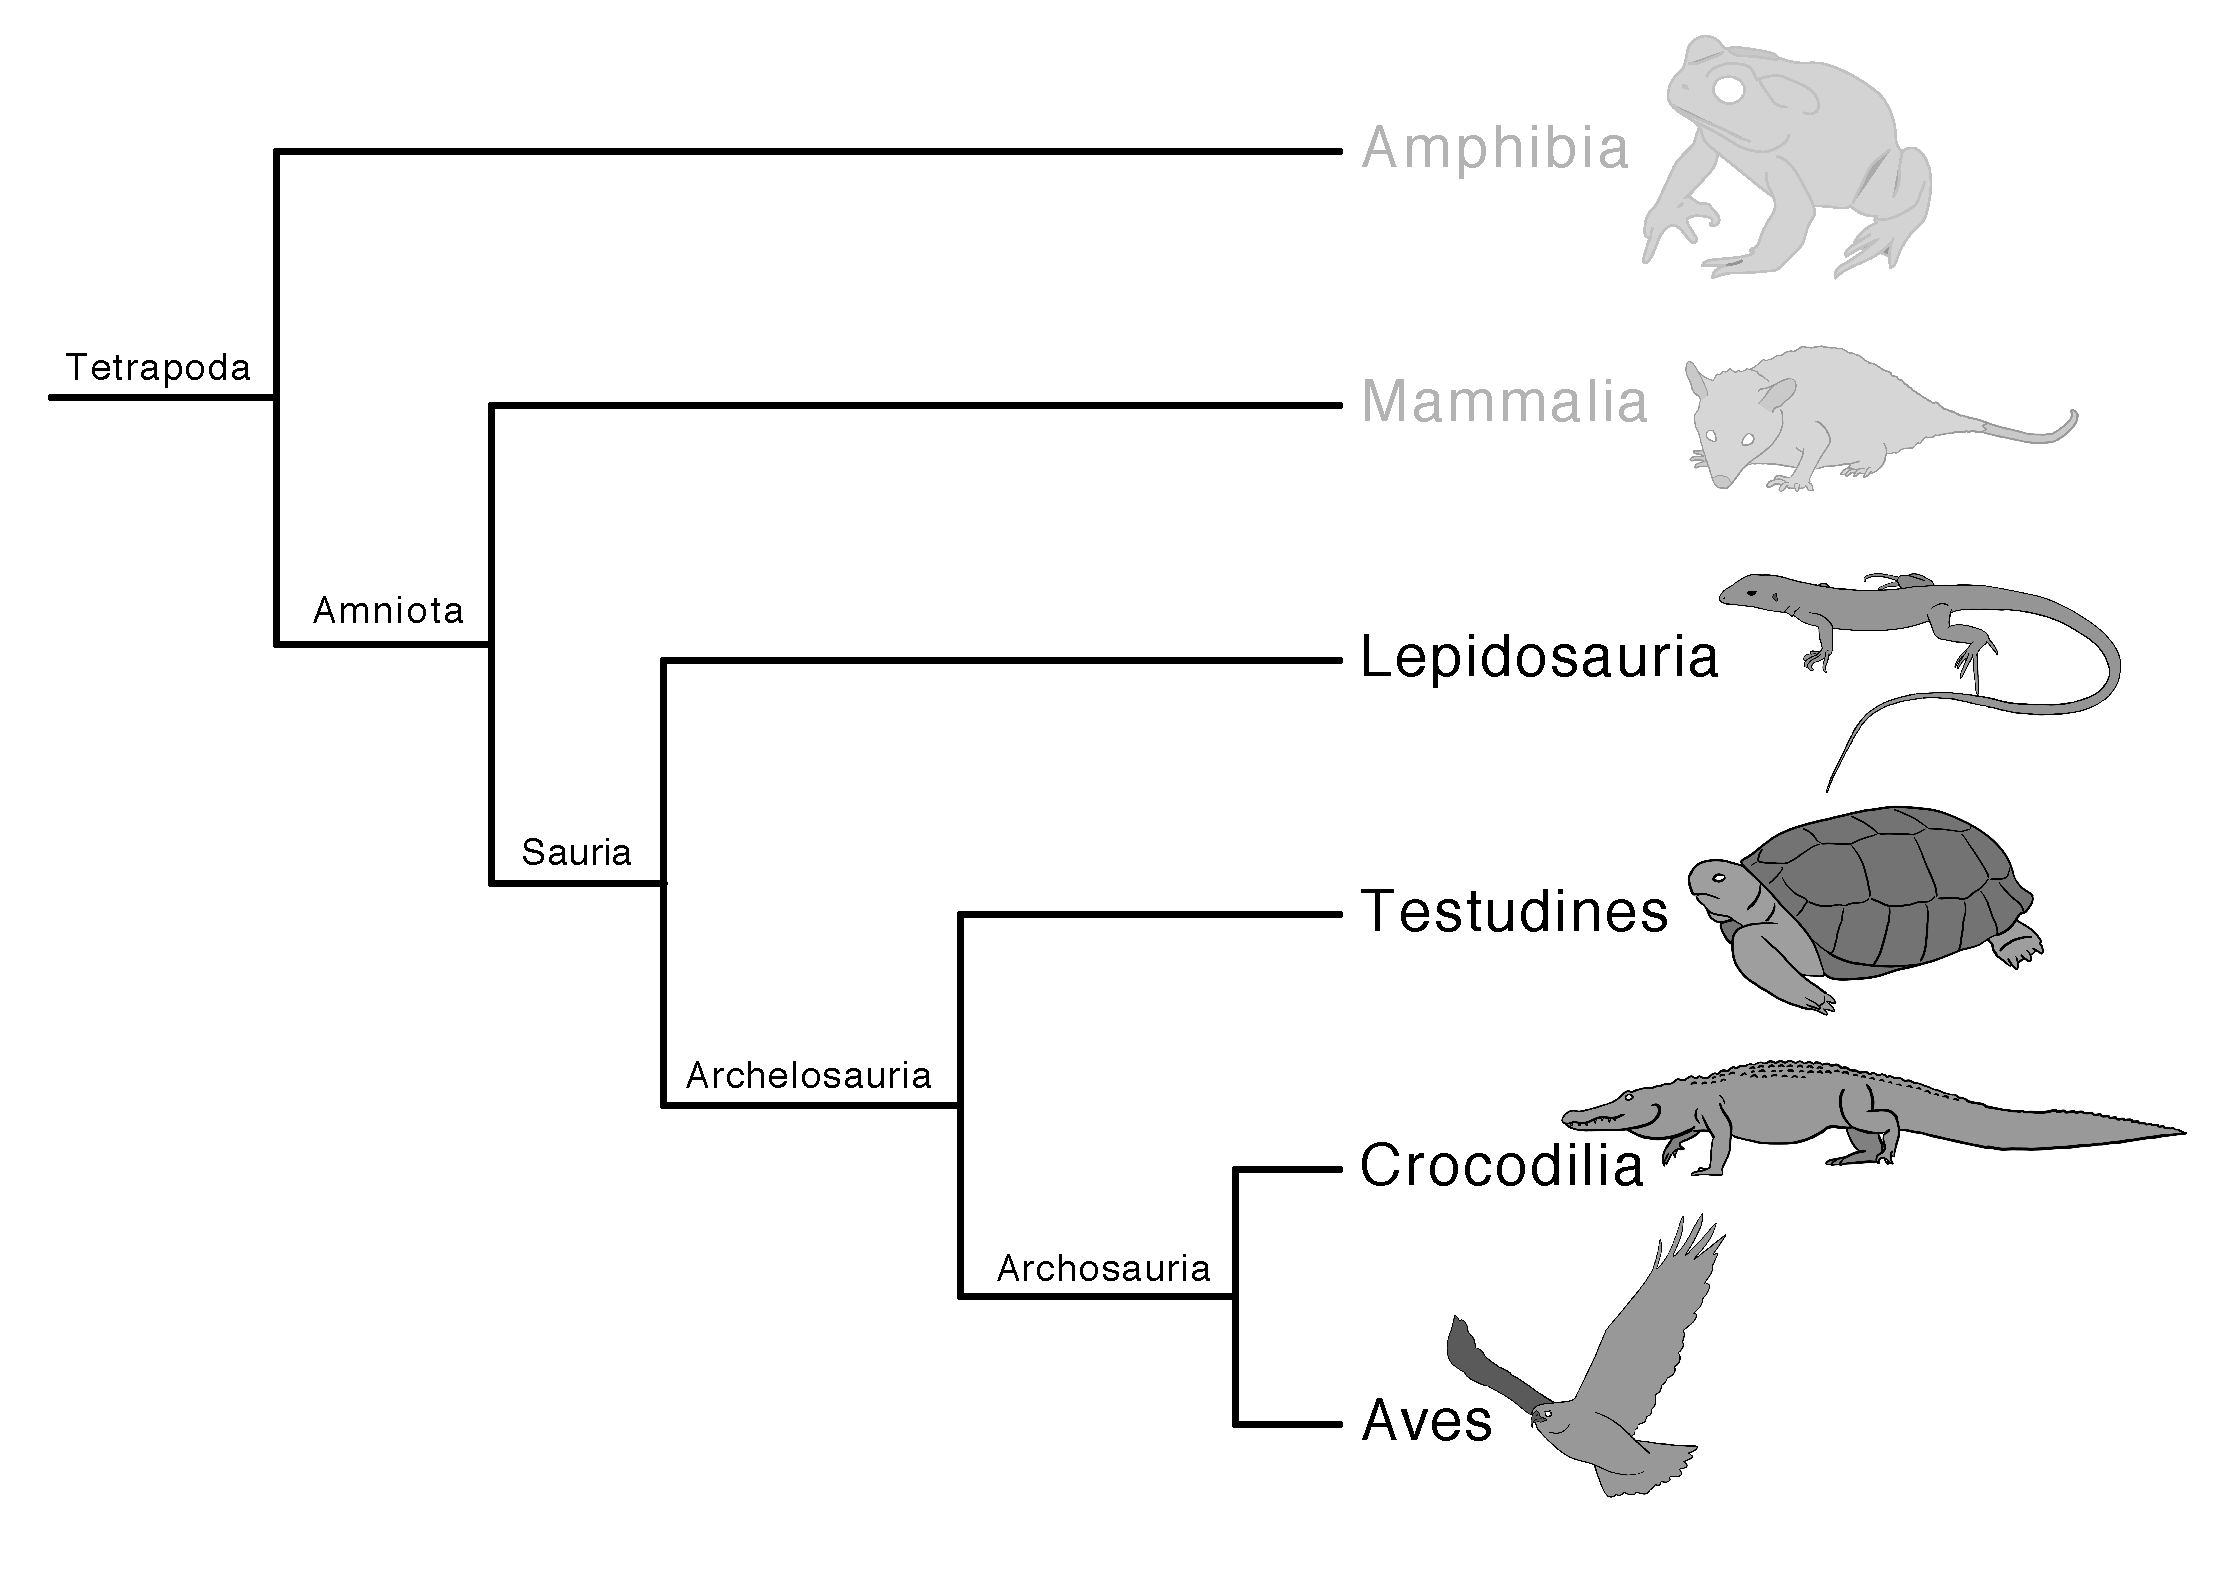
\includegraphics[scale=0.3]{Amniota_tre.pdf}
  \caption{Amniote Relationships}
  \label{fig:Amniota}
\end{figure}


\section{Lepidosauria}
Lab Reading: Simões et al., 2018. (Nature Letters) - Know Fig. 2 \\
Transverse cloacal slit, regular cycles of shedding, tongue distally notched, paired copulatory organs, well-developed quadrate conch, ectepicondylar foramen in the humerus (median nerve and brachial artery passage), pleurodont dentition

\begin{figure}[H]
\centering
  \includegraphics[scale=0.3]{Lepidosauria_tre_raw.pdf}
  \caption{Lepidosaur Relationships}
  \label{fig:Lepidosauria}
\end{figure}

\begin{description}
\item\textbf{Rhynchocephalia} \\ Once distributed globally (most abundant group in South America during Cretaceous). No well defined hemipenes- paired copulatory organs are slight outpushings of cloacal walls. Gastralia present.
\begin{itemize}
  \item Family {\textbf{SPHENODONTIDAE} (tuatara)} \\ Only extant Rhynchocelphalian (one genus, two species). Ancestral diapsid skull (two temporal fenestra on either side of skull). One or both of these holes have been lost in lizards and snakes, respectively. Highly developed pineal gland (regulates circadian rhythm). Teeth fused to skull (sphenodont dentition), and become dull with time. A single row of teeth on the lower jaw fit between two rows on the upper jaw, a trait unique among all tetrapods. Tuatara can live upwards of 100 years. * No alcohol-preserved specimen, just skull replicate.
\end{itemize}
\item\textbf{Squamata} \\ Highly developed hemipenes (paired copulatory organs), Jacobsen's organ separated from nasal capsule, femoral and preanal glands, no gastralia, triradiate squamosal
\begin{itemize}
  \item Family {\textbf{DIBAMIDAE} (blind skinks)} \\ In these elongate lizards, males have tiny flap like hindlimbs and females are completelylimbless. They also lack external ear openings. All of these features are likely adaptations totheir fossorial lifestyle. They are found in Mexico and in Southeast Asia. Largely limbless (small flap-like hindlimbs in males). * No specimen.
  \item{\textbf{Gekkota} (geckos)}
  \begin{itemize}
    \item Family {\textbf{GEKKONIDAE} (spectacled geckos)} \\ Two species have been introduced to Alabama. They are readily identified by their lack eyelids and setae-covered toe pads. Toe pads with tiny hair like structures called setae.. These toe pads enable them to climb vertical surfaces.
  \end{itemize}
  \item{\textbf{Scincoidea}}
  \begin{itemize}
    \item Family {\textbf{SCINCIDAE} (skinks)} \\ Dorsal scales smooth, shiny, and cicloid
  \end{itemize}
  \item{\textbf{Lacertoidea}} \\ Includes amphisbaenians, racerunners/whiptails, and tegus
  \begin{itemize}
    \item Family {\textbf{TEIIDAE}} \\ Have velvety textured dorsal scales and large, rectangular ventral scales, Pointed snout, Forked tougue, tail over 2x SVL, highly active foragers
  \end{itemize}
    \item{\textbf{Anguimorpha}} \\ Group that contains the only venemous lizards (Helodermatidae and Varanidae) and Anguids.
  \begin{itemize}
    \item Family {\textbf{ANGUIDAE}} \\ Elongate lizards with reduced limbs or limbless. Scales usually rectangular. Lateral fold in most taxa.
  \end{itemize}
  \item{\textbf{Iguania}} \\ Diverse group that includes acrodonts (Agamidae, Chamelonidae) and pleurodonts (Iguanidae, Corytophanidae, Crotaphytidae, and the following families)
  \begin{itemize}
    \item family {\textbf{DACTYLOIDAE}} \\ Have subdigital lamallae bearing setae much like gekkota. Males have prominent dewlaps.
    \item family {\textbf{PHRYNOSOMATIDAE}} (spiny lizards) \\ A number of species in this group have become important model species for ecology and physiology research. Many instances of viviparity.
  \end{itemize}
  \item{\textbf{Serpentes} (snakes)}
  \begin{itemize}
    \item grade {\textbf{LEPTOTYPHLOPIDAE}} \\ Burrowing snakes that eat termites. They are usually worm-like in appearance and cannot open their mouths widely.
    \item grade {\textbf{"Henophidia"}} \\ Paraphyletic grade that includes boas and pythons (which are also paraphyletic) along with several other groups of snakes.
    \item family {\textbf{VIPERIDAE}} (vipers) \\ Crotalinae (restricted to Eurasia \& Americas; all snakes listed below) have heat-sensing pit between eye and nostril; paired single tooth on maxilla (mobile fang) that functions to deliver potent venom (many species possess neurotoxic, hemotoxic, and cytotoxic venom- some with a cocktail), broad head, vertical pupil. Many species are viviparous.
    \item family {\textbf{ELAPIDAE}} (elapids) \\ Venomous snakes endemic to tropical and subtropical regions. Some snakes are aquatic (e.g., kraits). Longest venemous snake (king cobra). Fixed fangs at front of upper jaw for injecting venom, which is largely made up of neurotoxic compounds.
    \item family {\textbf{COLUBRIDAE}} \\ Lack heat-sensing pits; have multiple teeth onmaxilla. Make up 78\% of world’s snakespecies.

  \end{itemize}

  
\end{itemize}
\end{description}

\pagebreak

\section{Archelosauria}
While phylogenetic conclusions from morphological analyses conflict with those from genetic analyses, most systematists place testudines as sister to the group encompassing crocodylians and aves (archosauria). This larger group (archelosauria) lacks diagnostic anotomical characters, but thorough molecular data consistently recover the three groups together.

\begin{figure}[H]
\centering
  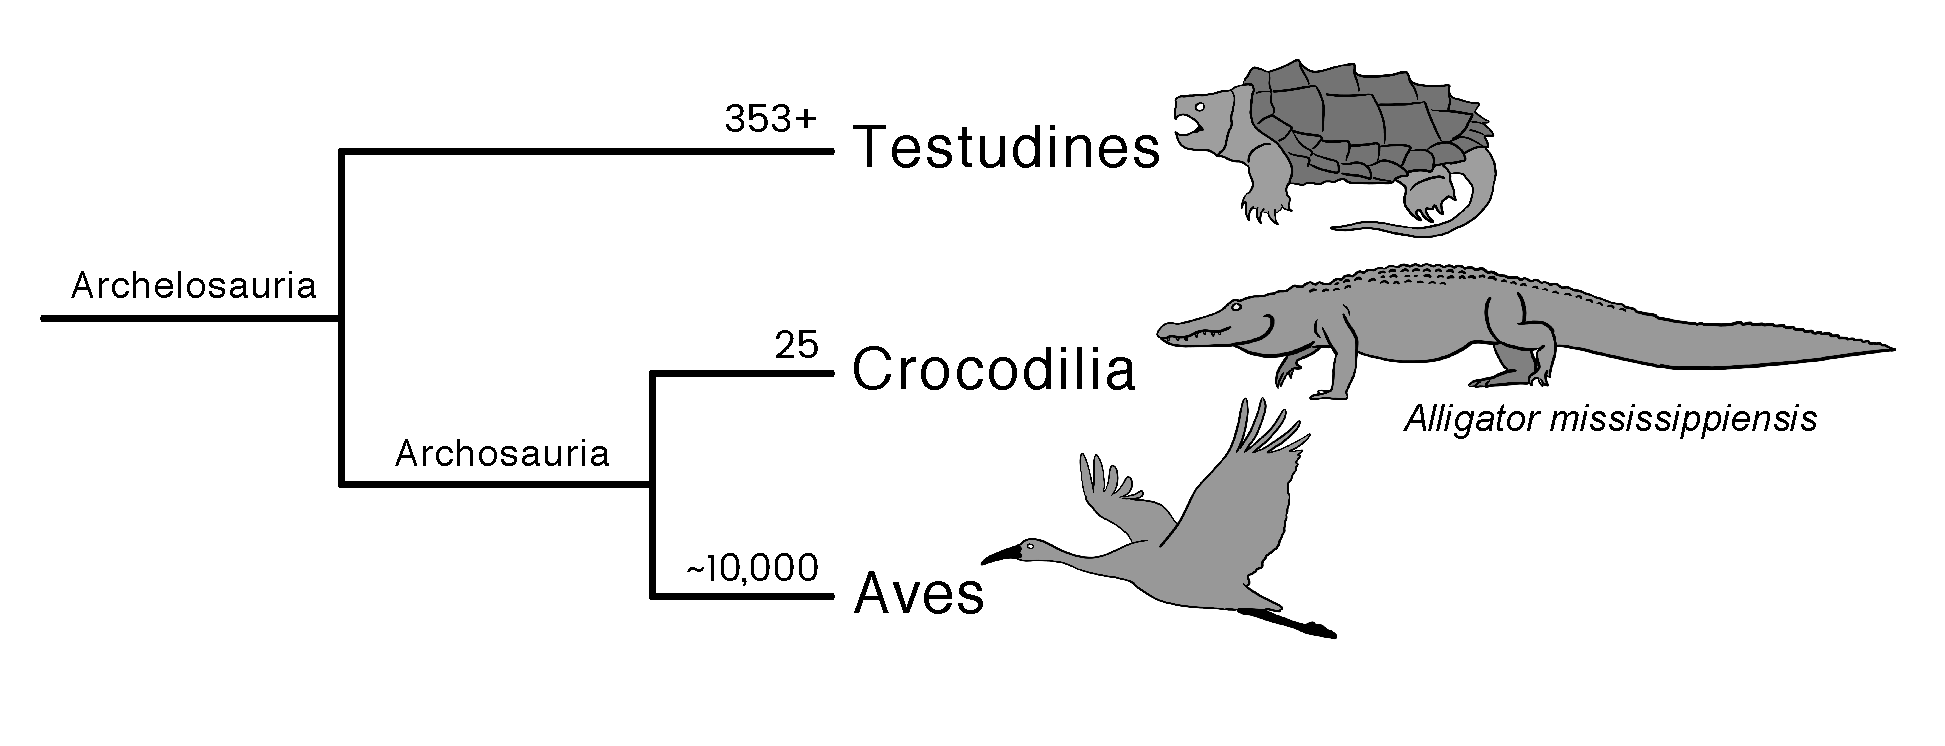
\includegraphics[scale=0.3]{Archelosauria_tre.pdf}
  \caption{Archelosaur Relationships}
  \label{fig:Archelosauria}
\end{figure}

\begin{description}
\item\textbf{Testudines} \\ Reptilian tanks- no other tetrapod with bony shell that encloses the pectoral and pelvic girdles. The carapace (dorsal portion of the shell) is made up of 8 trunk vertebrae fused with ribs and overlying dermal bones. The plastron (ventral portion of the shell) is made up of the sternum and gastralia fused with external dermal bones. The neck is made up of 8 cervical vertebrae. All turtles are oviparous with internal fertilization, and many have temperature-dependent sex determination.

\begin{figure}[H]
\centering
  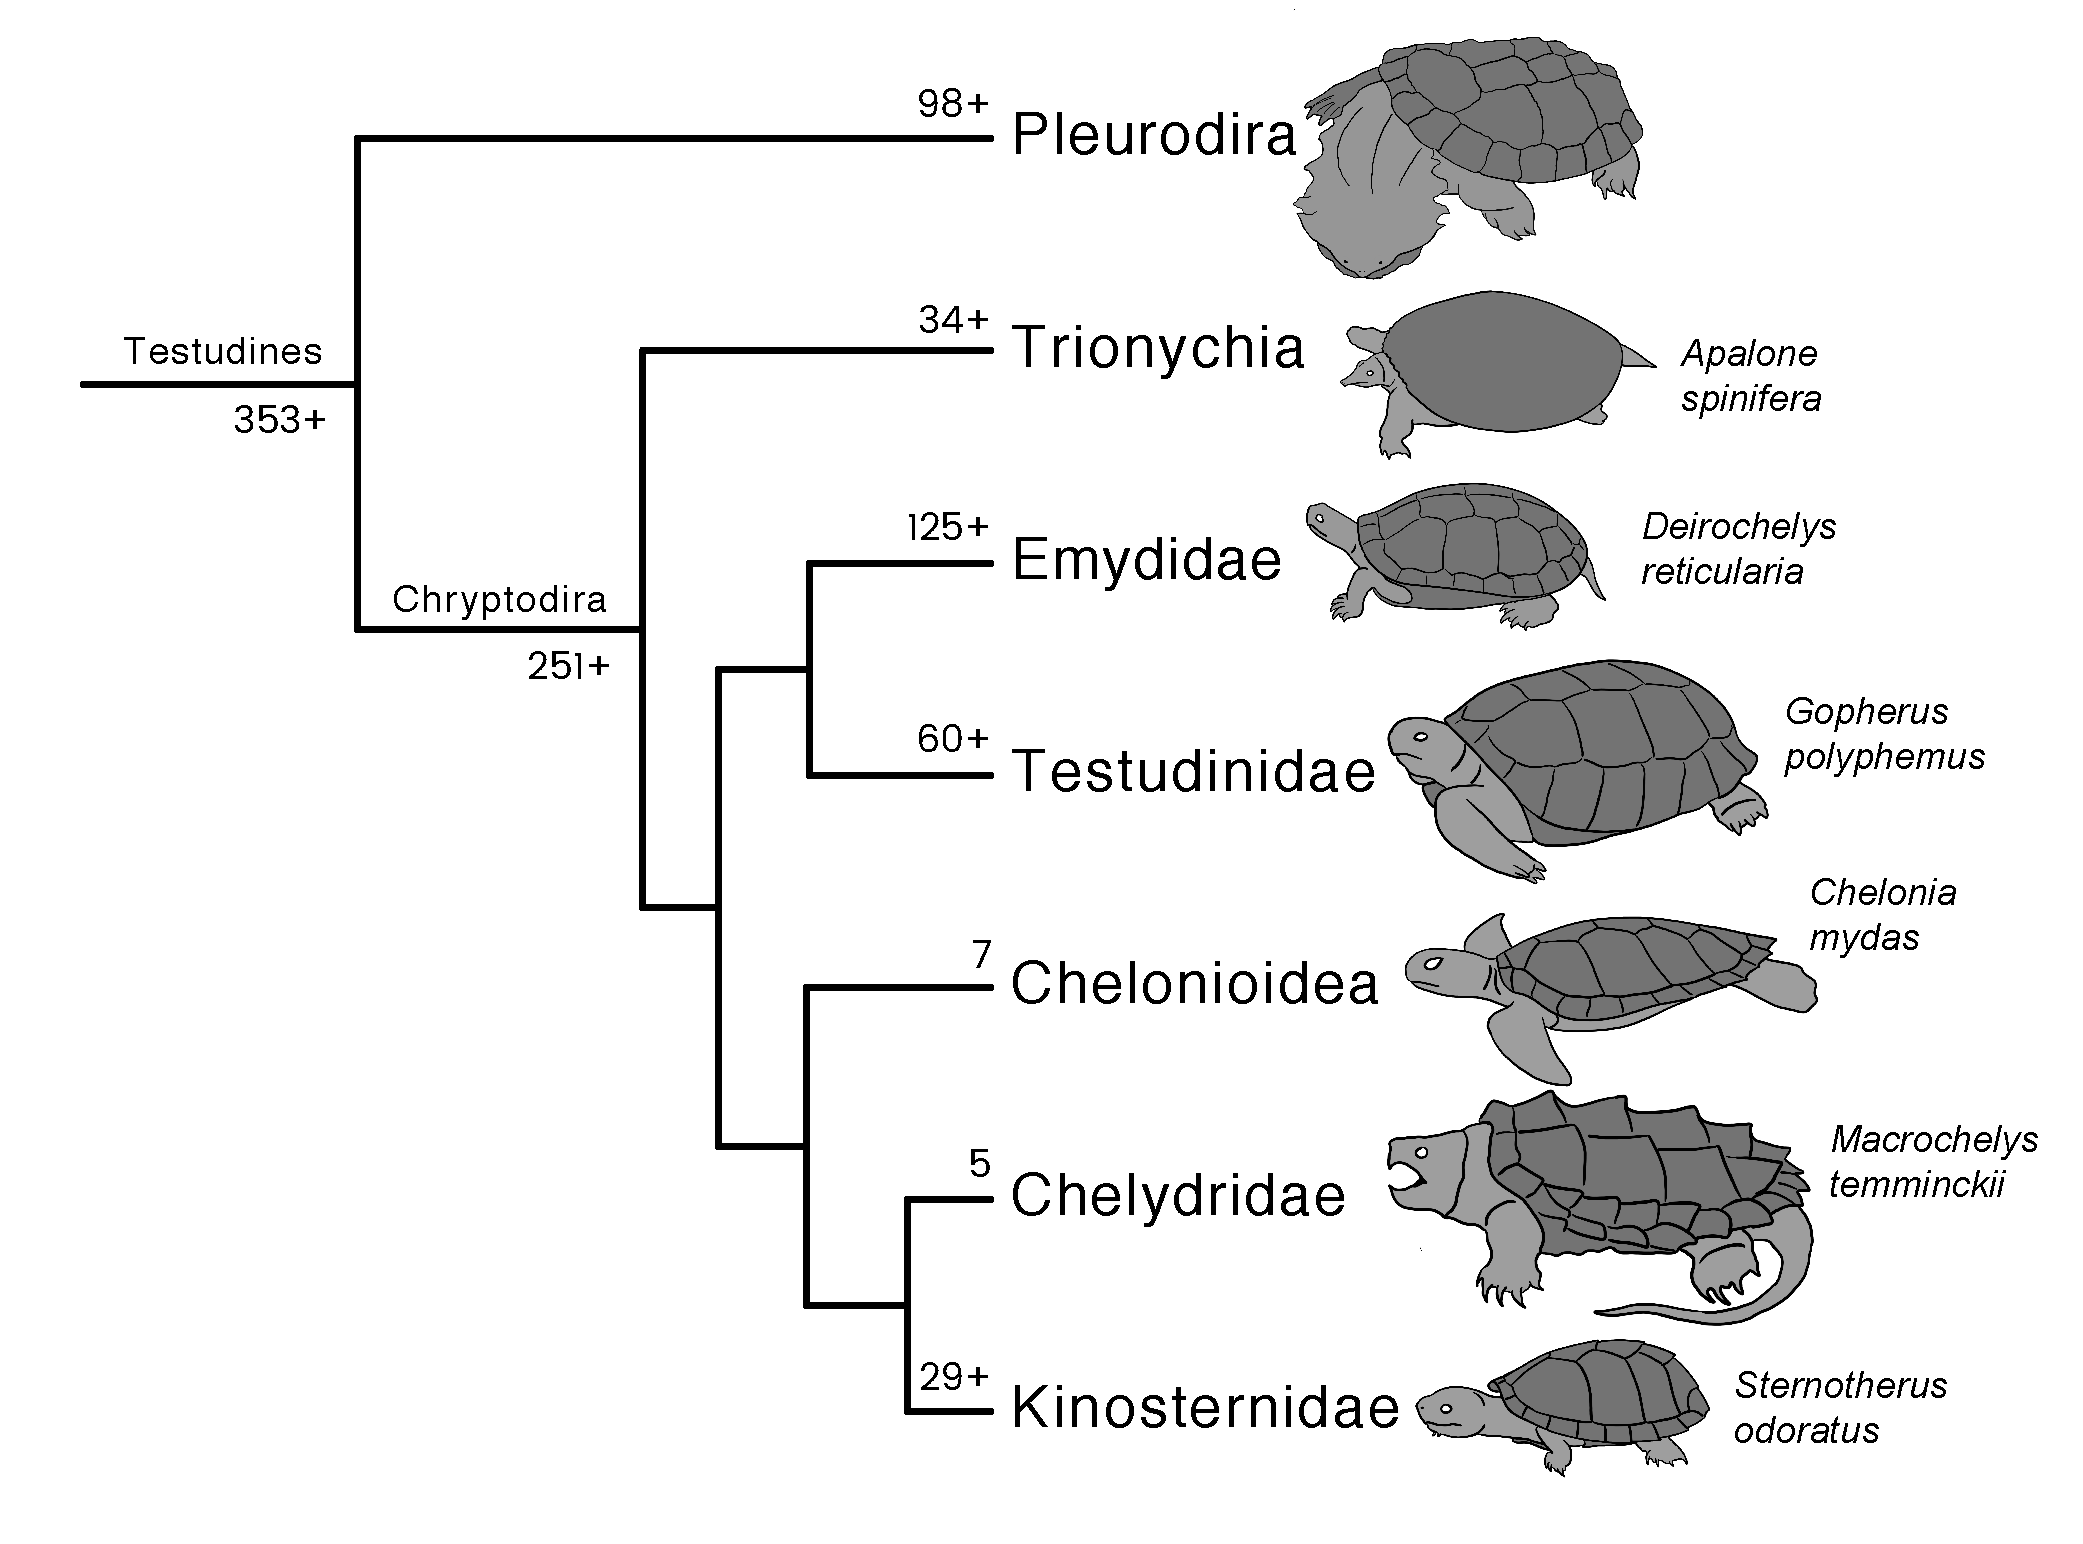
\includegraphics[scale=0.3]{Testudines_tre.pdf}
  \caption{Testudine Relationships}
  \label{fig:Testudines}
\end{figure}

\begin{itemize}
  \item{\textbf{Pleurodira} (side-neck turtles)} \\ Withdraw head and neck laterally within the outer margin of the shell
  \item{\textbf{Cryptodira} (S-neck turtles)} \\ Withdraw head and neck within shell in S-shape
  \begin{itemize}
    \item {\textbf{Trionychia} (softshell turtles)} \\ Flat, pancake shells, no epidermal scutes
    \item Family {\textbf{EMYDIDAE} (pond turtles)} \\ Moderately domed carapace, tear-drop shaped carapace
    \item Family {\textbf{TESTUDINIDAE} (tortoises)} \\ Terrestrial; forelimbs shovel-like for digging, hind feet elephantine for walking.
    \item {\textbf{CHELONIOIDEA} (sea turtles)} \\ Limbs modified into flippers, streamlined shell
    \item {\textbf{CHELYDRIDAE} (snapping turtles)} \\ Large head, flattened carapace, long tails (about as long as carapace)
    \item {\textbf{KINOSTERNIDAE} (mud and musk turtles)} \\ Plastron with 10 or 11 scutes, defined overhanging beak, potato-like (oblong) shape
  \end{itemize}
\end{itemize}
\end{description}

\begin{description}
\item\textbf{Crocodilia} \\ Robust skull, long snout, strongly toothed jaws, short neck, robust cylindrical trunk, laterally compressed tail, short but strongly developed limbs with webbed feet. Largest living reptiles. Bony plates (osteoderms) covered by keratinou skin provide armor to neck, trunk, and tail. All crocodylians are oviparous with internal fertilization, and have temperature-dependent sex determination. 

\begin{figure}[H]
\centering
  \includegraphics[scale=0.3]{Crocodilia_tre.pdf}
  \caption{Crocodilian Relationships}
  \label{fig:Crocodilia}
\end{figure}

\begin{itemize}
  \item Family {\textbf{ALLIGATORIDAE}} \\ Broad snout, mostly new world distribution (one exception in alligatorinae)
  \begin{itemize}
    \item {\textbf{Alligatorinae} (alligators)} \\ Two extant species (Eastern China and North America)
    \item {\textbf{Caimaninae} (caiman)} \\ New world distribution (Central and South America). Fourth mandibular tooth exposed when mouth closed. * No specimen
  \end{itemize}
  \item Family {\textbf{GAVIALIDAE} (gharials)} \\ Long, slender snout (fish eaters). Asian distribution. * No specimen
  \item Family {\textbf{CROCODYLIDAE} (crocodiles)} \\ Global distribution, relatively narrow snout.
\end{itemize}


\end{description}

\end{document}

